\section{与退休养老资产的协整关系}
由于美国FOF基金的兴起, 主要源于养老金市场的发展. 美国雇员逐渐选择将养老金计划由DB(Defined Benefit) Plan转向DC(Defined Contribute) Plan, 增大了养老金投资着的投资需求. 而FOF基金作为一种收益稳定、风险二次分散的基金, 自然受到了这些被动投资者的青睐. 下面, 利用彭博数据库中FOF基金资产总量和养老金资产总量的季度数据, 对FOF基金市场与养老金市场进行协整分析. 在2007--2016十年中, 二者的绝对数量和增长率变化趋势如下:

% 两个市场的趋势图像
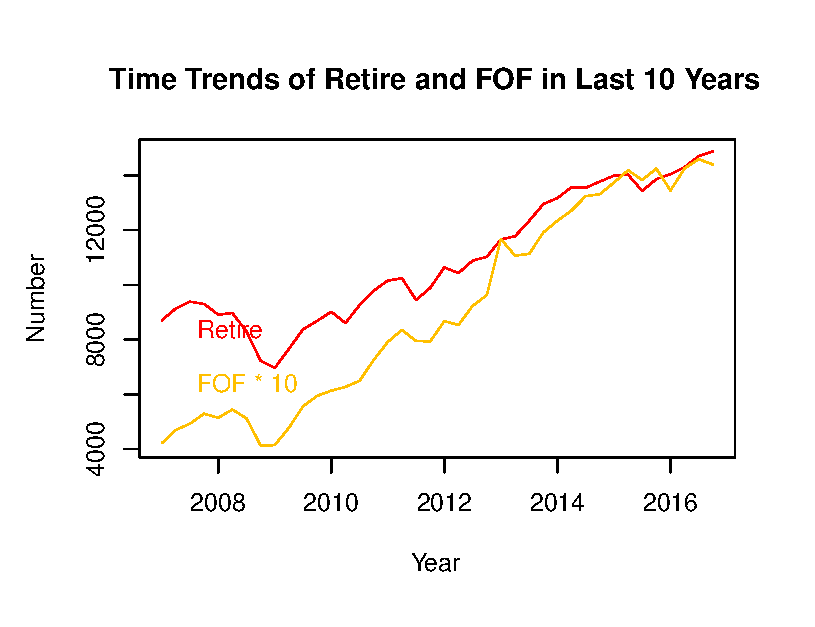
\includegraphics[width=0.4\textwidth]{pic/3-0-1.eps}
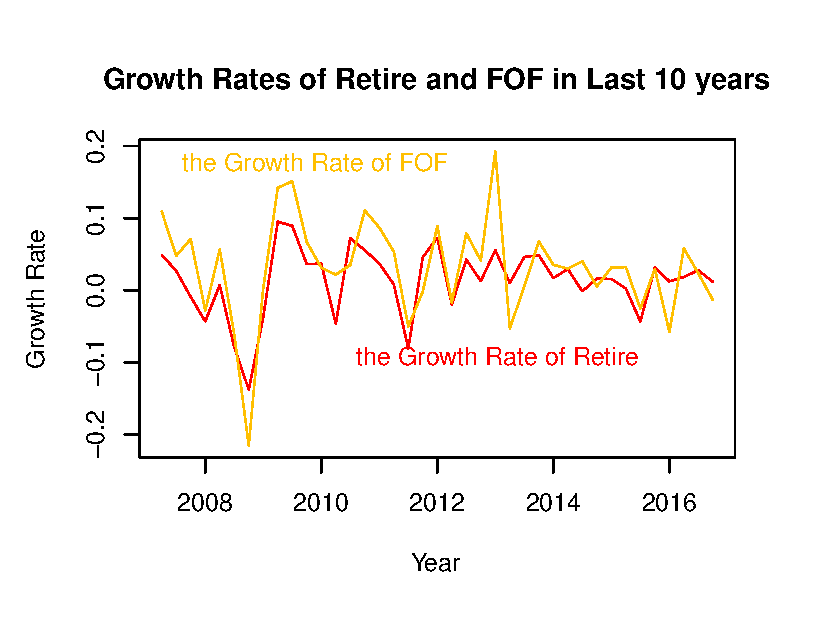
\includegraphics[width=0.4\textwidth]{pic/3-0-2.eps}

\textcolor{red}{修改:将图片按照引言里的格式插入,对照代码即可,可能会需要subfigure命令,可以参考tex源文件里下面隐藏着的被注释掉的代码,by RQJ}

%\begin{figure}[ht]
%  \centering
%  \subfigure[Small Box with a Long Caption]{
%    \label{fig:subfig:a} %% label for first subfigure
%    \includegraphics[width=1.0in]{pic1.eps}}
%  \hspace{1in}
%  \subfigure[Big Box]{
%    \label{fig:subfig:b} %% label for second subfigure
%    \includegraphics[width=1.5in]{pic.eps}}
%  \caption{Two Subfigures}
%  \label{fig:subfig} %% label for entire figure
%\end{figure}

% 单位根检验部分
对${FOF_t}$和${Retire_t}$序列分别进行单位根检验. ADF检验和Phillips–Perron的结果接受了原假设(单位根过程), 并且Kwiatkowski–Phillips–Schmidt–Shin检验结果拒绝了原假设(平稳过程). 因此可以认为${FOF_t}$和${Retire_t}$是非平稳序列.
继续对它们的差分序列${\Delta FOF_t}$和${\Delta Retire_t}$进行单位根检验, 得到的结果表明它们是平稳序列. 所以, ${FOF_t}$和${Retire_t}$分别是2个$I(1)$序列. 下面对这两个序列进行协整估计.

% 协整部分
首先, 使用最小二乘法估计如下方程:
$$FOF_t = \alpha + \beta \cdot Retire_t + \mu_t$$
得到$\alpha$和$\beta$的估计量$\hat{\alpha}$和$\hat{\beta}$. 估计结果如表~\ref{tab:coin-OLS-estimate}~所示.

% OLS回归结果表格
\begin{table}[ht]
    \centering
    \caption{OLS估计量}
    \label{tab:coin-OLS-estimate}
    \begin{tabular}{l | rrrr}
        Coefficients: &            &            &         &                     \\
                      & Estimate   & Std. Error & t value & Pr(\textgreater|t|) \\  \hline
        (Intercept)   & -7.552e+02 & 5.632e+01  & -13.41  & 5.51e-16***        \\
        Retire        & 1.524e-01  & 5.042e-03  & 30.22   & \textless 2e-16***
    \end{tabular}
\end{table}


对残差估计序列$\hat{\mu}_t$进行单位根检验, $\hat{\mu}_t$在ADF检验和PP检验中拒绝了存在单位根的原假设, 在KPSS检验中接受了序列平稳的原假设.
因此可以认为${FOF_t}$和${Retire_t}$两个$I(1)$过程得到了平稳的$I(0)$
过程. 即两个序列之间存在着长期的均衡关系(协整关系). 协整向量为$(1, -0.15)$, 表~\ref{tab:coin-OLS-resid-uniroot}~所示.

% 残差具有平稳性
\begin{table}[ht]
    \centering
    \caption{OLS估计残差的单位根检验}
    \label{tab:coin-OLS-resid-uniroot}
    \begin{tabular}{l | cccc}
        Tests        & ADF-Test       & KPSS-Test      & PP-Test               \\  \hline
        Statistics   & -3.1799 (<1pct) & 0.2674(<10pct) & -10.0379 (<Z-tau)
    \end{tabular}
\end{table}

% Error Correction Model
记$y_t = FOF_t$, $x_t = Retire_t$, 建立误差修正模型. 由于使用的是季度数据, 所以加入$\Delta y_t$的1-4阶滞后项.
$$\Delta y_t = \alpha_1 \cdot \Delta y_{t-1} + \alpha_2  \cdot \Delta  y_{t-2} + \alpha_3 \cdot \Delta  y_{t-3} + \alpha_4 \cdot \Delta  y_{t-4} + \beta_0 \cdot \Delta  x_t+\beta_1 \cdot \Delta  x_{t-1} + +\gamma \cdot ( y_{t-1}-kx_{t-1}) + \epsilon_t$$

\textcolor{red}{修改: 上面式子里连续有两个加号?仔细检查一下有没有缺项少项的问题,by任庆杰}

估计结果表~\ref{tab:coin-correction-model}~所示.
\begin{table}[ht]
    \centering
    \caption{误差修正模型估计结果}
    \label{tab:coin-correction-model}
    \begin{tabular}{l | rrrr}
        Coefficients: &          &            &         &                     \\
                      & Estimate & Std. Error & t value & Pr(\textgreater|t|) \\  \hline
        (Intercept)   & 22.13335 & 11.14436   & 1.986   & 0.0573              \\
        L(y, 1)       & -0.46108 & 0.19994    & -2.306  & 0.029*             \\
        L(y, 2)       & -0.01601 & 0.12908    & -0.124  & 0.9022              \\
        L(y, 3)       & -0.03563 & 0.12999    & -0.274  & 0.7861              \\
        L(y, 4)       & -0.02875 & 0.13862    & -0.207  & 0.8373              \\
        L(x, 1)       & 0.05842  & 0.02549    & 2.292   & 0.03*              \\
        L(x, 0)       & 0.09517  & 0.01852    & 5.138   & 0.000021***        \\
        L(r, 1)       & -0.38373 & 0.16855    & -2.277  & 0.0309*
    \end{tabular}
\end{table}


误差修正项的系数在10\%的程度显著, 协整向量为$(1, -0.15)$.

\textcolor{red}{补充: 几句话说明建立误差修正模型的原因及其能说明的问题,by RQJ}
